 \documentclass[a4paper,12pt]{article}

\usepackage{graphicx}
\usepackage[absolute,overlay]{textpos}
\usepackage{anyfontsize}
\usepackage{etoolbox}
\usepackage{array}
\usepackage{longtable}
\usepackage{caption}
\usepackage{geometry}
\geometry
{ a4paper,
  total={170mm,250mm},
  left=20 mm,
  right=20mm,
  top=25mm ,
  bottom=20mm}
\def\doubleunderline#1{\underline{\underline{#1}}}

\makeatletter
\patchcmd{\@maketitle}{\vskip 2em}{\vspace*{-2cm}}{}{}
\makeatother

\pagenumbering{gobble}

%Code Colors&Features
\usepackage{listings}
\usepackage{xcolor}

\definecolor{codegreen}{rgb}{0,0.6,0}
\definecolor{codegray}{rgb}{0.5,0.5,0.5}
\definecolor{codepurple}{rgb}{0.58,0,0.82}
\definecolor{backcolour}{rgb}{0.95,0.95,0.92}

\lstdefinestyle{mystyle}{
    backgroundcolor=\color{backcolour},   
    commentstyle=\color{codegreen},
    keywordstyle=\color{magenta},
    numberstyle=\tiny\color{codegray},
    stringstyle=\color{codepurple},
    basicstyle=\ttfamily\footnotesize,
    breakatwhitespace=false,         
    breaklines=true,                 
    captionpos=b,                    
    keepspaces=true,                 
    numbers=left,                    
    numbersep=5pt,                  
    showspaces=false,                
    showstringspaces=false,
    showtabs=false,                  
    tabsize=2
}

\lstset{style=mystyle}


\usepackage{makeidx}
\makeindex


\begin{document}

\title { \large \textsc{Università degli Studi di Napoli Federico II \\
		 Scuola Politecnica e delle Scienze di Base} \\
\textsc{Dipartimento di Ingegneria Elettrica e Tecnologie dell’Informazione}}

\author{}
\date{}
\maketitle 
\thispagestyle{empty}

\vspace*{-2cm}
\begin{center}
	\begin{figure}[h]
	\centering
 	
\includegraphics[width=0.3\textwidth]{unina_logo.png}
	\end{figure}
	
	\Large \textsc{Corso di laurea in Informatica \\
		   Insegnamento di Object Orientation\\
		   Anno Accademico 2019-2020}
\end{center}

\vspace*{+1.5cm}
\begin{center}
\Huge \bf Documentazione di un software gestionale per recensioni turistiche
\end{center}


\vspace*{-2cm}
\vfill 
\begin{flushleft}
\textit{Autori:} \hfill \textit{Docente:}


\normalsize{\textsc{Davide Pio Faicchia} \hfill \normalsize{Prof. Sergio \textsc{DI MARTINO}}


\textsc{MATRICOLA : N86003018 }


\textit{da.faicchia@studenti.unina.it}}

\end{flushleft}


\begin{flushleft}
\normalsize{\textsc{Mauro Guida}


\textsc{MATRICOLA : N86002889}


\textit{maur.guida@studenti.unina.it}}
\end{flushleft}



\newpage\null\thispagestyle{empty}
\begin{center}
\vfil
\vfil
\textit{Questa pagina è stata lasciata intenzionalmente bianca. } 
\vfil
\vfil 
\end{center}
\newpage

\newpage\null\pagenumbering{arabic}\setcounter{page}{3}
\begin{flushleft}
\vspace*{+1cm}
\begingroup
\fontsize{35pt}{12pt}\selectfont\bf{Indice}
\endgroup
\vspace*{+1cm}

\Large\textsc{\bf Capitolo 1 - ClassDiagram} \hfill 4\\

\Large\textsc{\bf Capitolo 2 - Sequence Diagrams} \hfill 5\\
\hspace{+1cm}\large 2.1 generaRisultatiHomepage \hfill 5\\
\hspace{+1cm}\large 2.2 impostaPassword \hfill 6\\
\hspace{+1cm}\large 2.3 ProcediInPubblicaBusiness3\hfill 7\\
\hspace{+1cm}\large 2.4 loginSchermataAccesso\hfill 8\\
\hspace{+1cm}\large 2.5 invioEmailCodiceVerificaSchermataAccessoReimpostaPassword \hfill 9\\

\Large\textsc{\bf Capitolo 3 - MockUp }\hfill 10\\

\end{flushleft}
\newpage

\newpage\null\pagenumbering{arabic}\setcounter{page}{4}

\begin{flushleft}

\Large\textsc{\bf Capitolo 1}
\vspace*{+1cm}

\begingroup
\fontsize{35pt}{12pt}\selectfont\bf{Class Diagram}
\endgroup
\vspace*{+1cm}

\begin{center}
	\begin{figure}[h]
	\centering
 	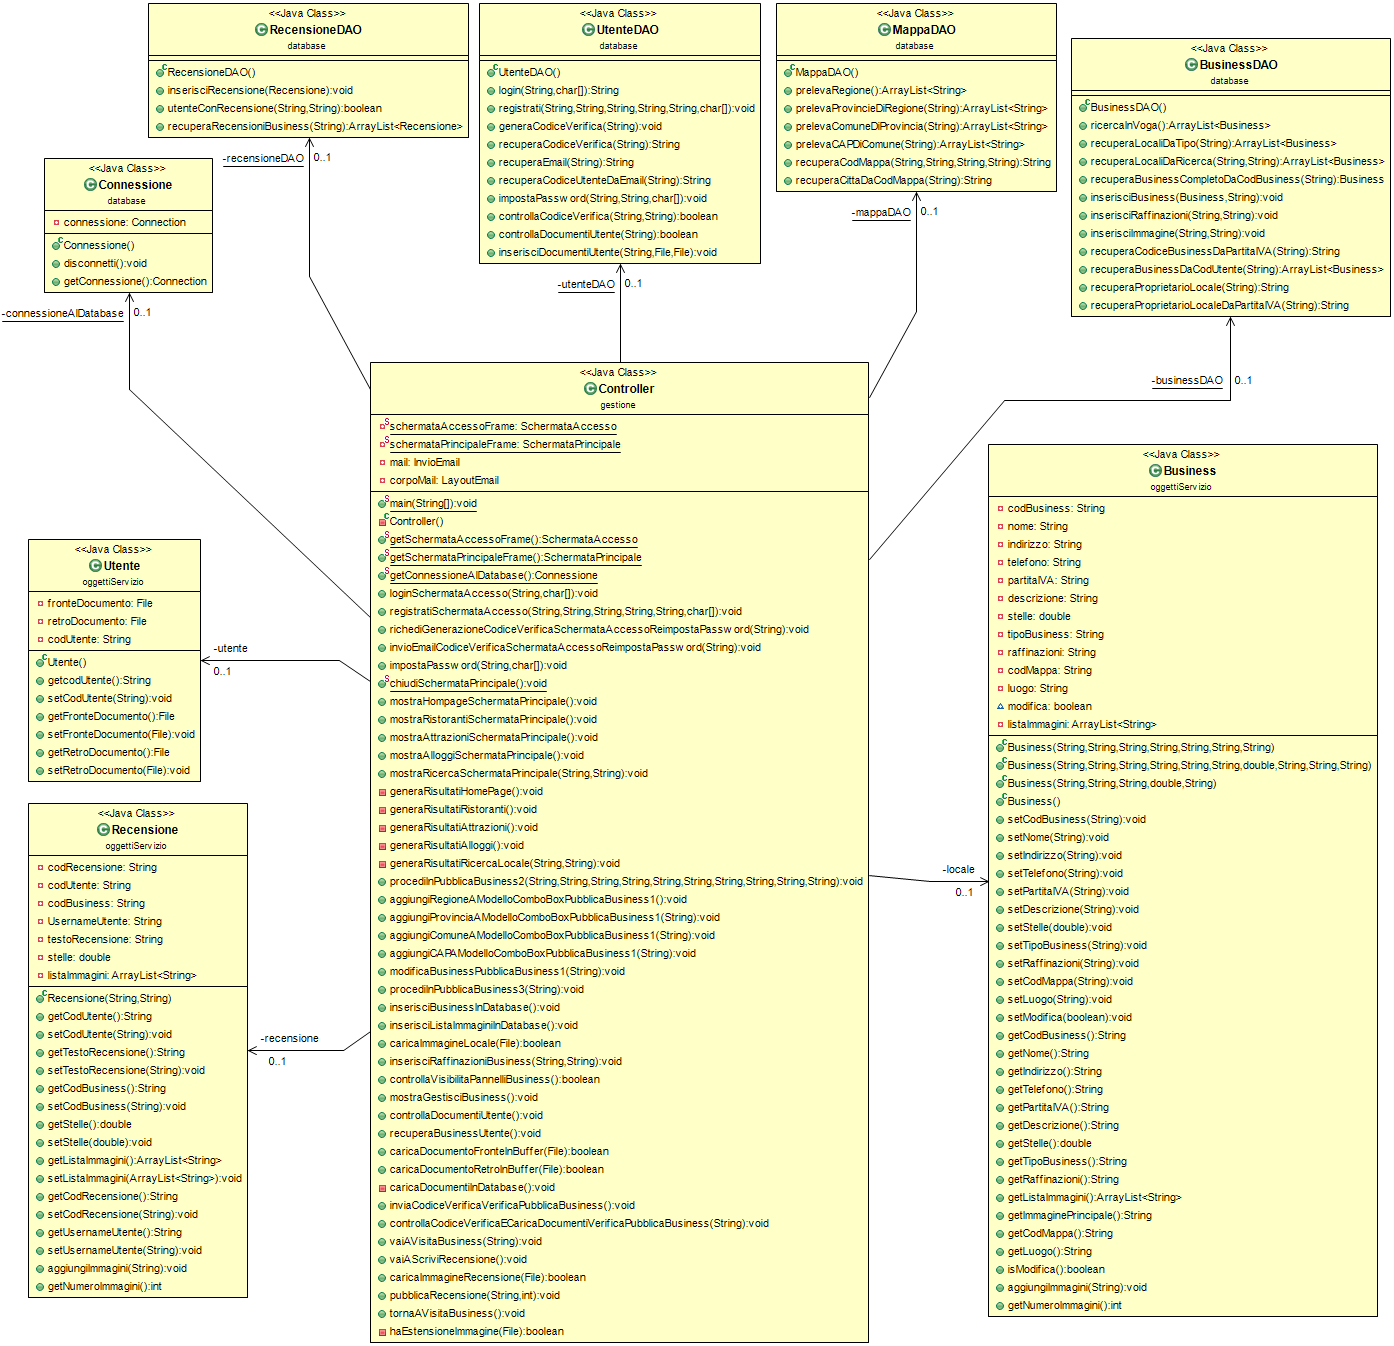
\includegraphics[width=1\textwidth]{ClassDiagram.png}
	\end{figure}
\end{center}


\normalsize{\it{*Gli identificatori delle associazioni rappresentano una determinata istanza di quella classe nel controller}}
\end{flushleft}
\newpage

\newpage\null\pagenumbering{arabic}\setcounter{page}{5}
\begin{flushleft}

\vspace*{+1cm}
\Large\textsc{\bf Capitolo 2}
\vspace*{+1cm}

\begingroup
\fontsize{35pt}{12pt}\selectfont\bf{Sequence Diagrams}
\endgroup
\vspace*{+1cm}

{\bf\normalsize 2.1 Metodo generaRisultatiHomepage }
\begin{center}
	\begin{figure}[h]
	\centering
 	\includegraphics[width=1\textwidth]{generaRisultatiHomepage.jpg}
	\end{figure}
\end{center}
\end{flushleft}
\newpage

\newpage\null\pagenumbering{arabic}\setcounter{page}{6}
\begin{flushleft}
\vspace*{+2cm}
{\bf\normalsize 2.2 Metodo impostaPassword }
\begin{center}
	\begin{figure}[h]
	\centering
 	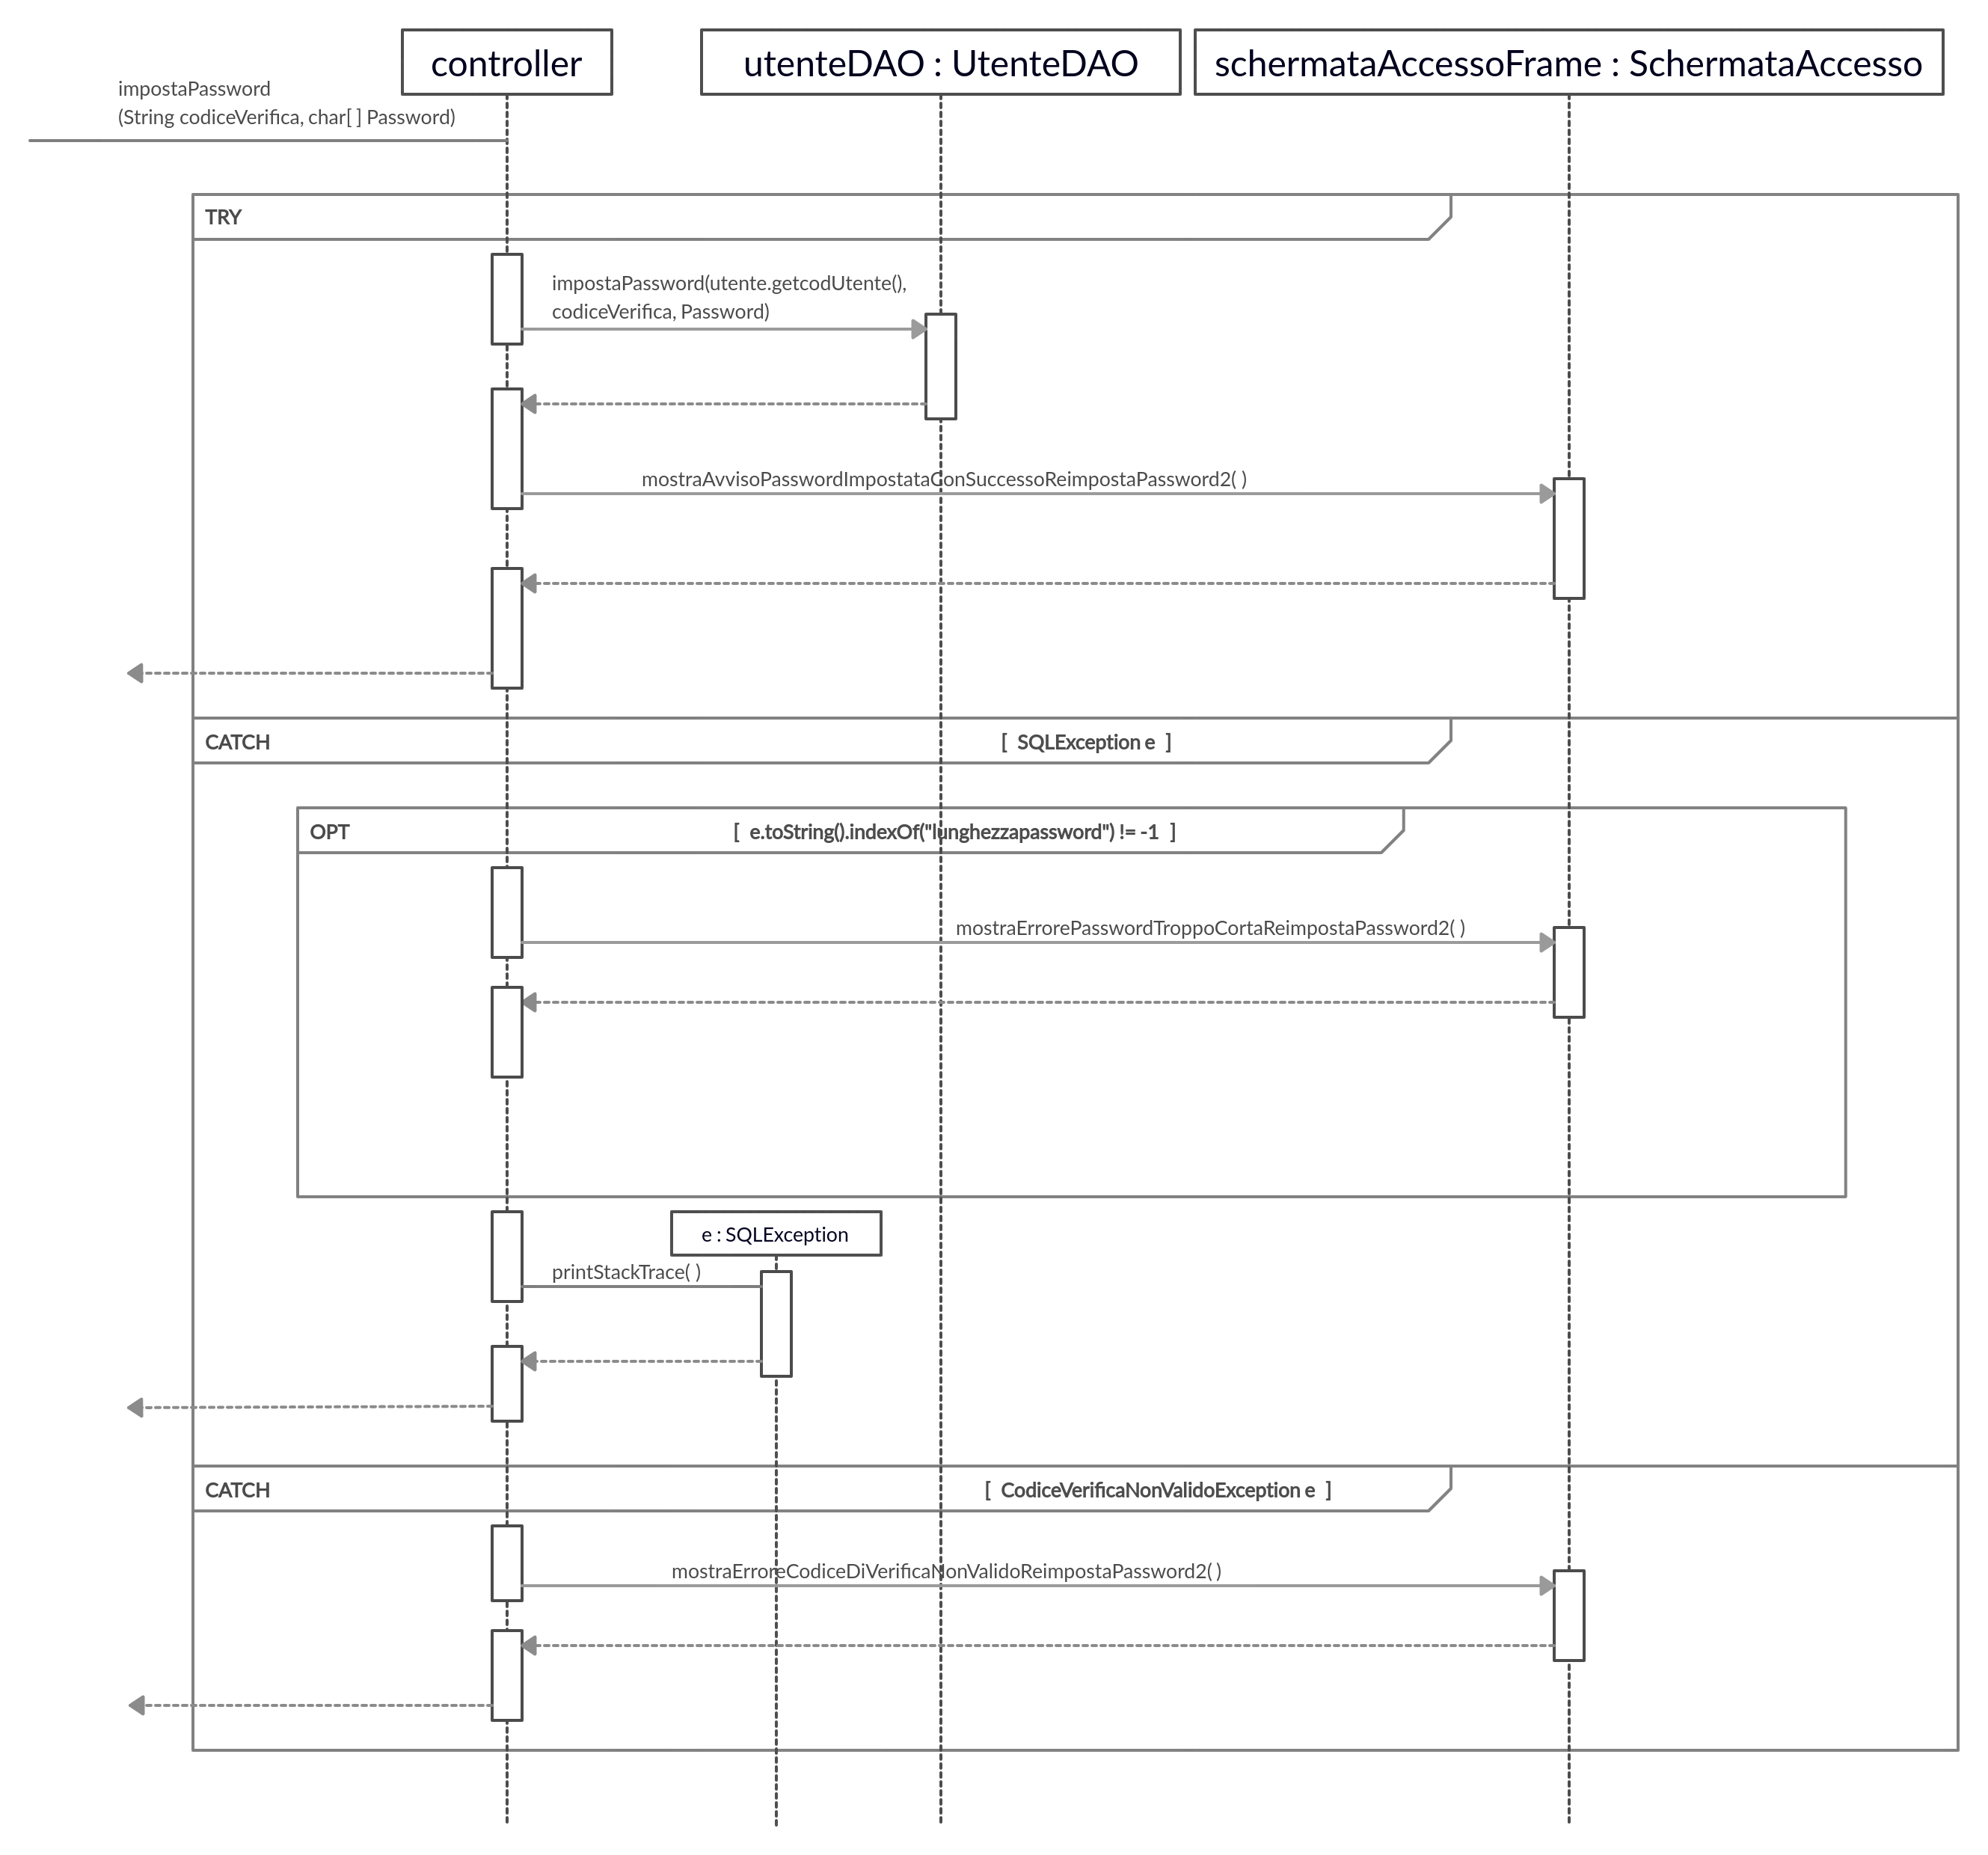
\includegraphics[width=1\textwidth]{impostaPassword.jpg}
	\end{figure}
\end{center}
\end{flushleft}
\newpage

\newpage\null\pagenumbering{arabic}\setcounter{page}{7}
\begin{flushleft}
\vspace*{+1cm}
{\bf\normalsize 2.3 Metodo ProcediInPubblicaBusiness3 }
\begin{center}
	\begin{figure}[h]
	\centering
 	\includegraphics[width=1\textwidth]{ProcediInPubblicaBusiness3.jpg}
	\end{figure}
\end{center}
\end{flushleft}
\newpage

\newpage\null\pagenumbering{arabic}\setcounter{page}{8}
\begin{flushleft}
\vspace*{+1cm}
{\bf\normalsize 2.4 Metodo loginSchermataAccesso }
\begin{center}
	\begin{figure}[h]
	\centering
 	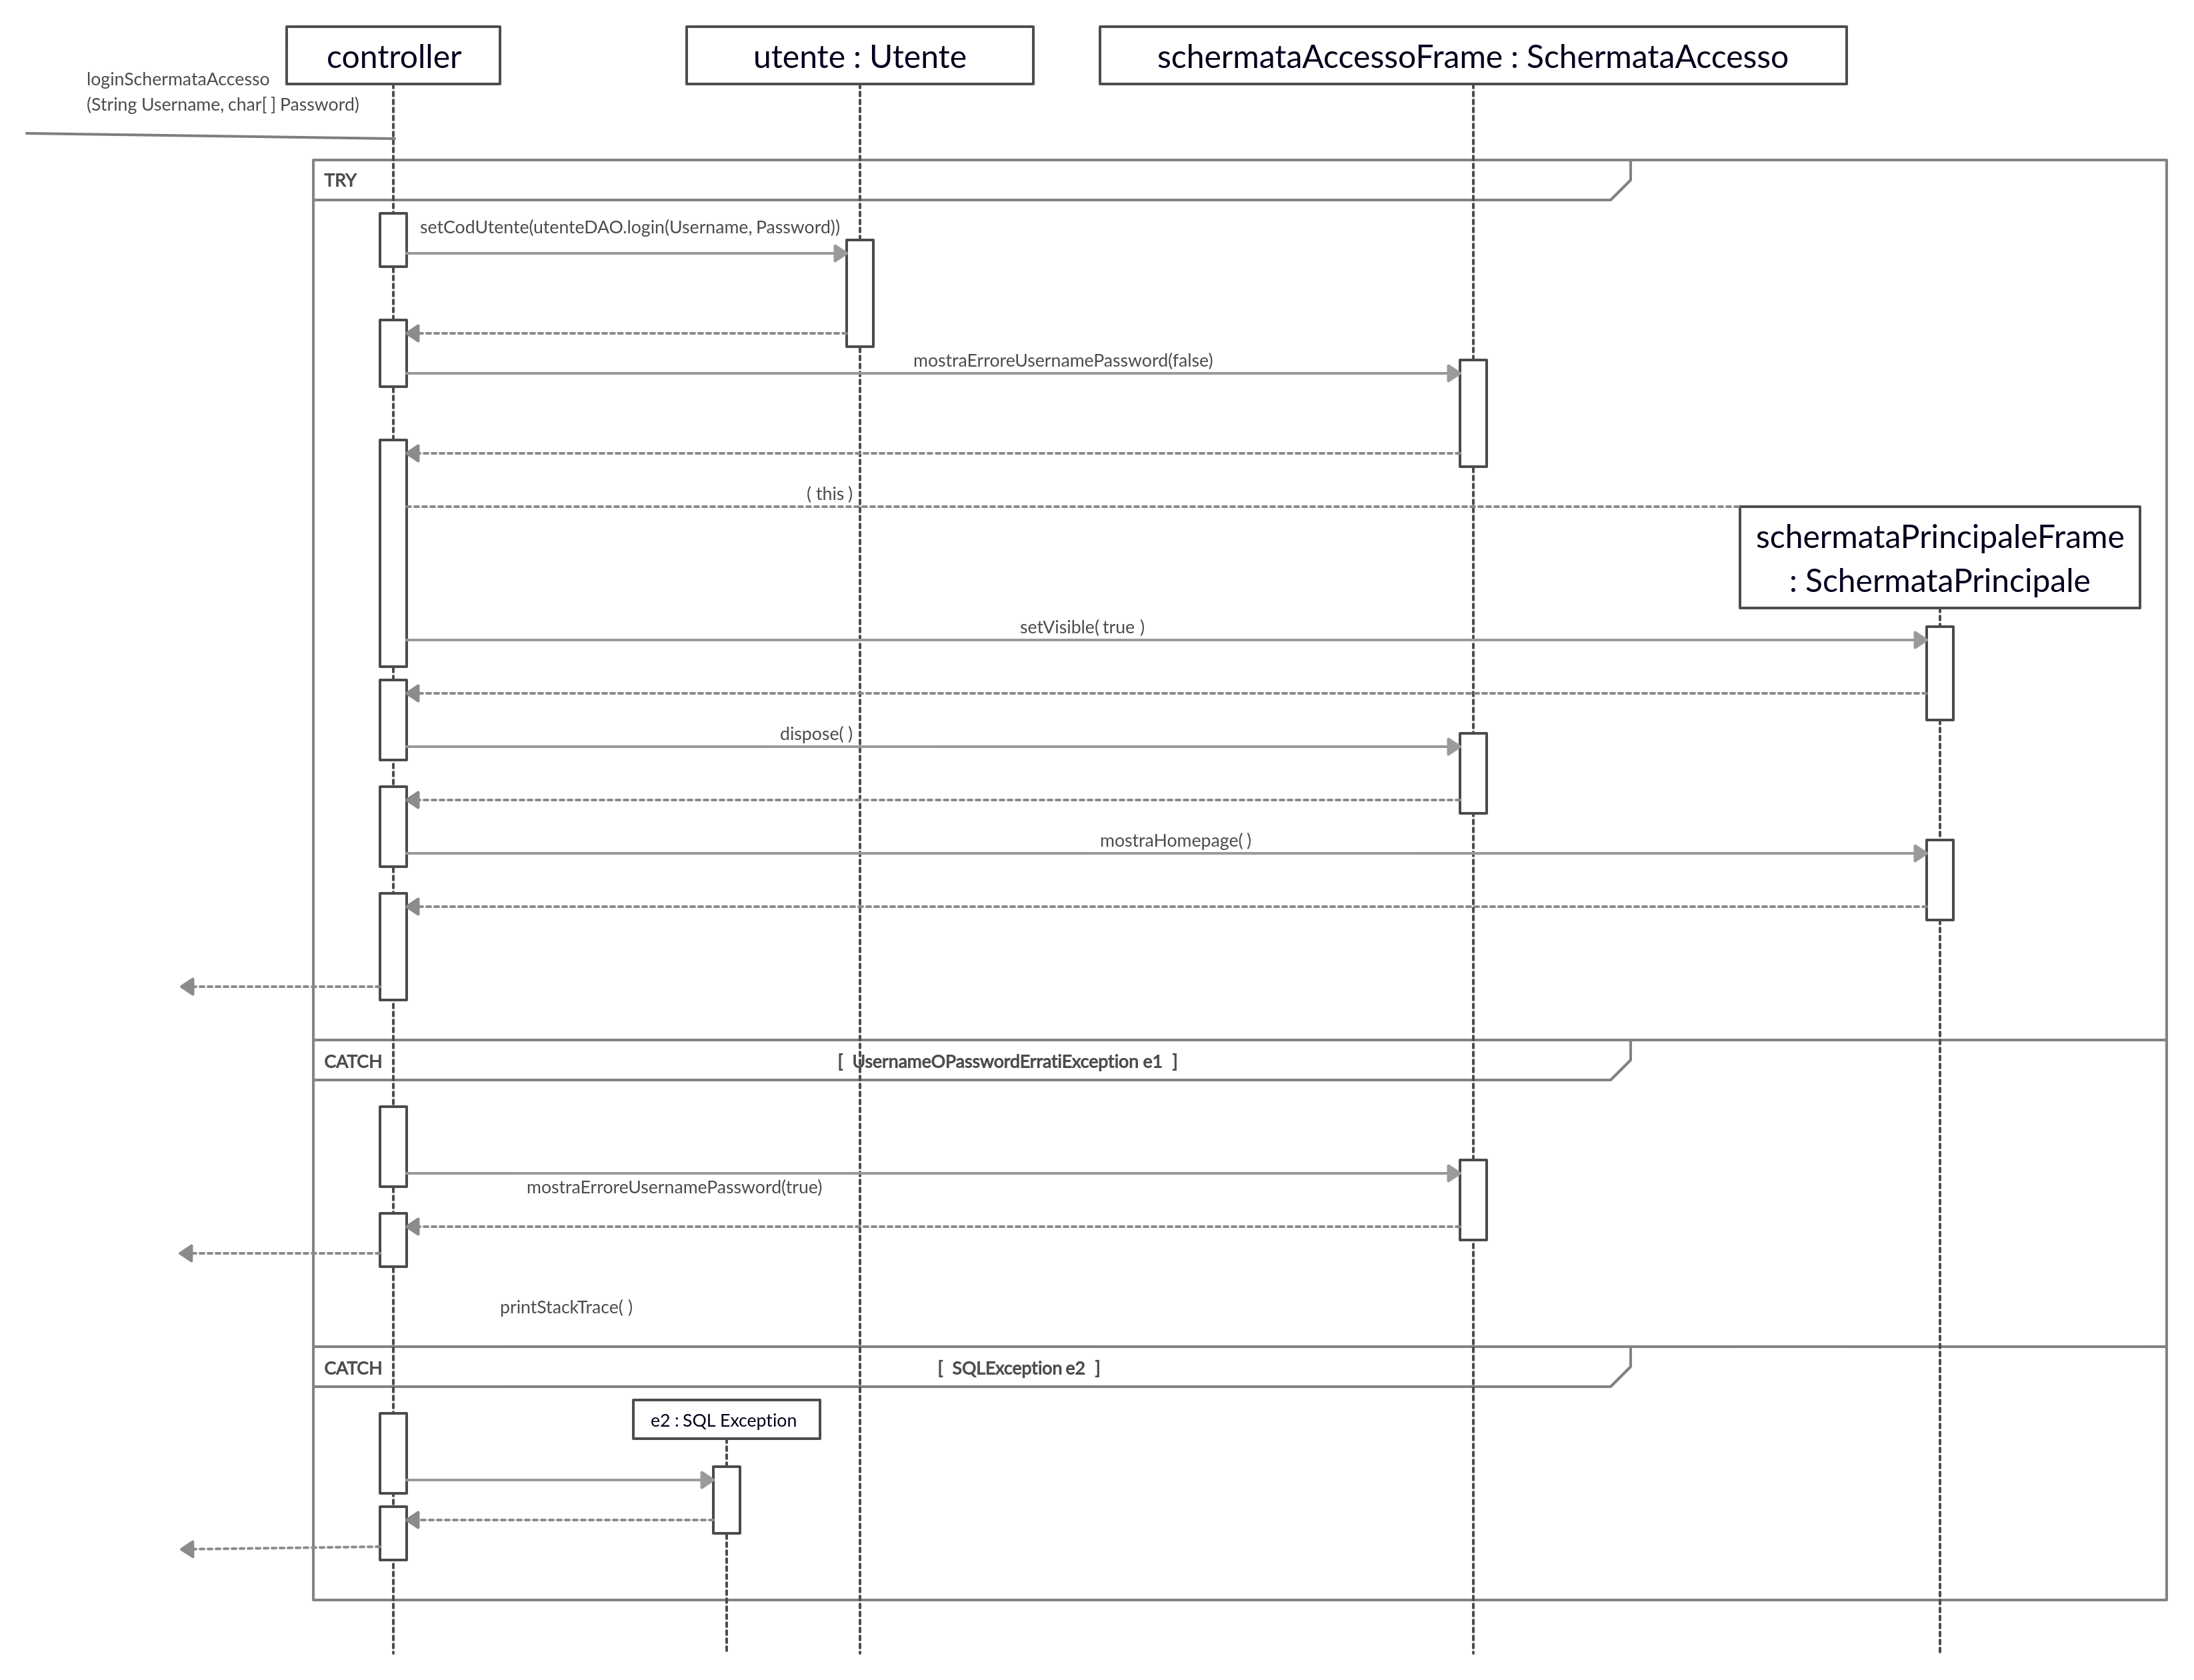
\includegraphics[width=1\textwidth]{loginSchermataAccesso.jpg}
	\end{figure}
\end{center}
\end{flushleft}
\newpage

\newpage\null\pagenumbering{arabic}\setcounter{page}{9}
\begin{flushleft}
\vspace*{+2cm}
{\bf\normalsize 2.5 Metodo invioEmailCodiceVerificaSchermataAccessoReimpostaPassword }
\begin{center}
	\begin{figure}[h]
	\centering
 	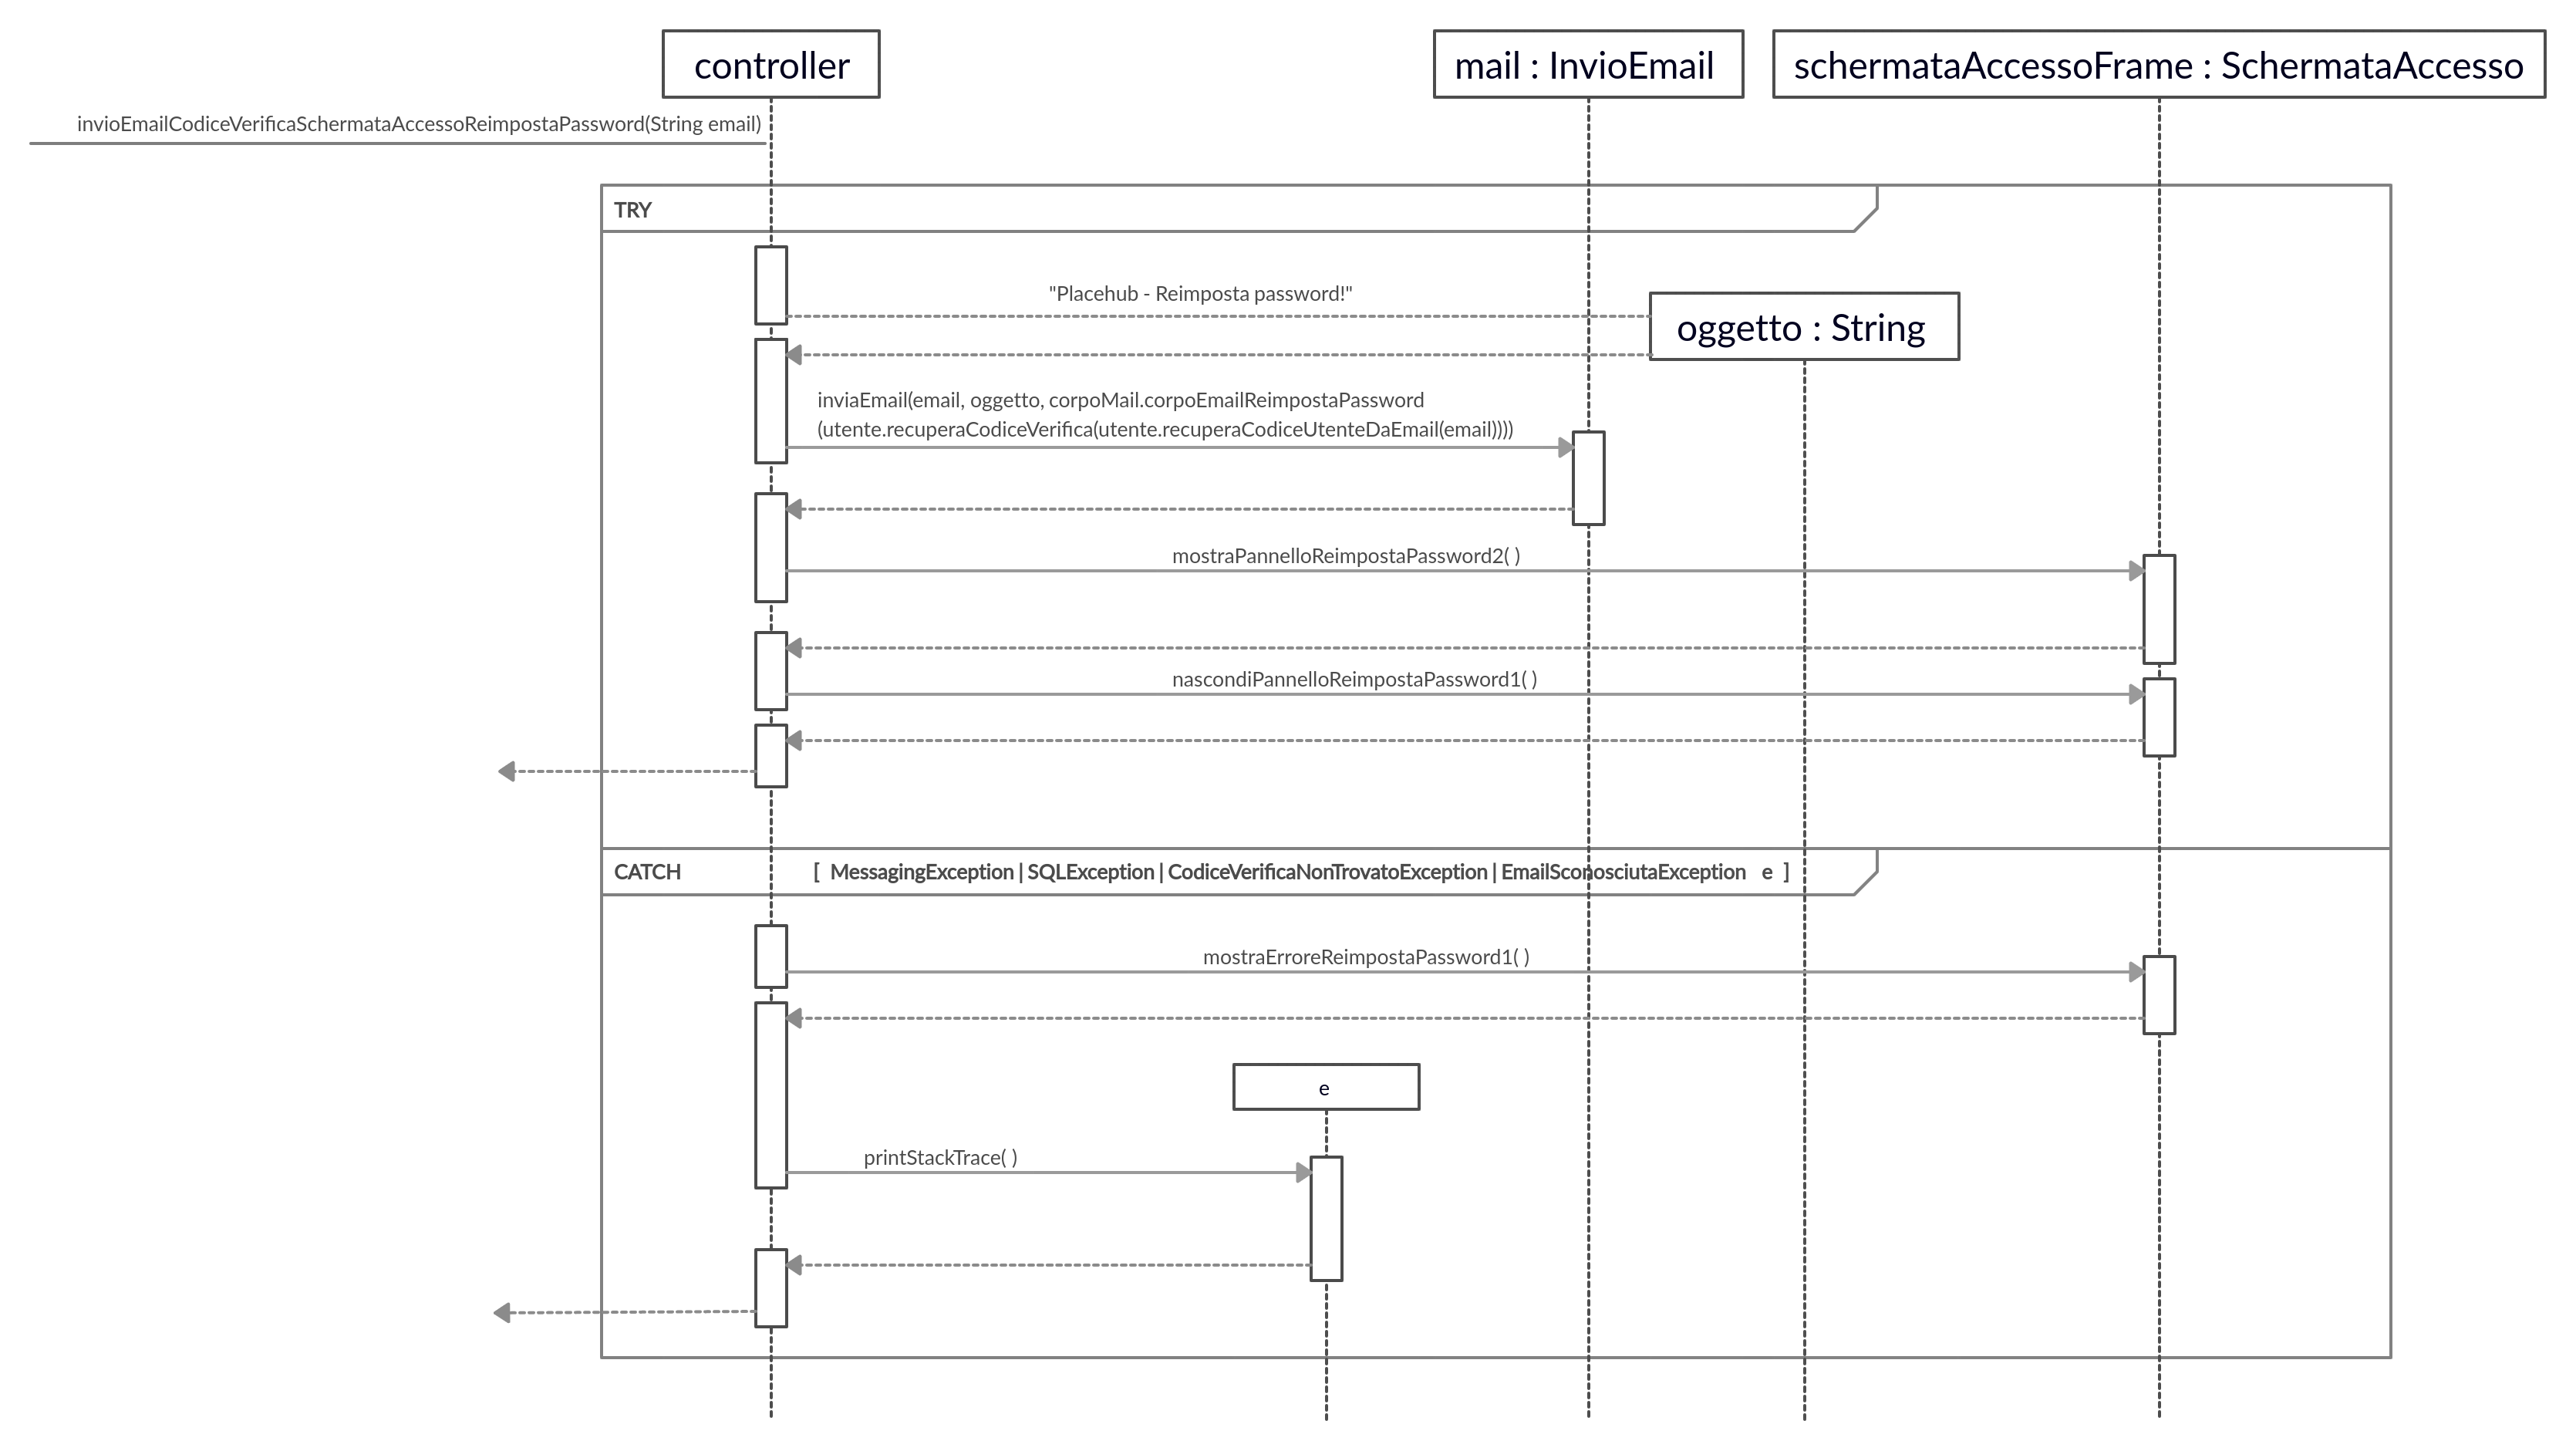
\includegraphics[width=1\textwidth]{invioEmailCodiceVerificaSchermataAccessoReimpostaPassword.jpg}
	\end{figure}
\end{center}
\end{flushleft}
\newpage

\newpage\null\pagenumbering{arabic}\setcounter{page}{10}
\vspace*{+1cm}
\Large\textsc{\bf Capitolo 3}
\vspace*{+1cm}

\begingroup
\fontsize{35pt}{12pt}\selectfont\bf{MockUp}
\endgroup
\vspace*{+2cm}
\begin{center}
\normalsize{\it{*vedi prossima pagina}}
\end{center}

\newpage

\end{document}